% Options for packages loaded elsewhere
\PassOptionsToPackage{unicode}{hyperref}
\PassOptionsToPackage{hyphens}{url}
%
\documentclass[
  11pt,
]{article}
\usepackage{amsmath,amssymb}
\usepackage{iftex}
\ifPDFTeX
  \usepackage[T1]{fontenc}
  \usepackage[utf8]{inputenc}
  \usepackage{textcomp} % provide euro and other symbols
\else % if luatex or xetex
  \usepackage{unicode-math} % this also loads fontspec
  \defaultfontfeatures{Scale=MatchLowercase}
  \defaultfontfeatures[\rmfamily]{Ligatures=TeX,Scale=1}
\fi
\usepackage{lmodern}
\ifPDFTeX\else
  % xetex/luatex font selection
\fi
% Use upquote if available, for straight quotes in verbatim environments
\IfFileExists{upquote.sty}{\usepackage{upquote}}{}
\IfFileExists{microtype.sty}{% use microtype if available
  \usepackage[]{microtype}
  \UseMicrotypeSet[protrusion]{basicmath} % disable protrusion for tt fonts
}{}
\makeatletter
\@ifundefined{KOMAClassName}{% if non-KOMA class
  \IfFileExists{parskip.sty}{%
    \usepackage{parskip}
  }{% else
    \setlength{\parindent}{0pt}
    \setlength{\parskip}{6pt plus 2pt minus 1pt}}
}{% if KOMA class
  \KOMAoptions{parskip=half}}
\makeatother
\usepackage{xcolor}
\usepackage[margin=1in]{geometry}
\usepackage{longtable,booktabs,array}
\usepackage{calc} % for calculating minipage widths
% Correct order of tables after \paragraph or \subparagraph
\usepackage{etoolbox}
\makeatletter
\patchcmd\longtable{\par}{\if@noskipsec\mbox{}\fi\par}{}{}
\makeatother
% Allow footnotes in longtable head/foot
\IfFileExists{footnotehyper.sty}{\usepackage{footnotehyper}}{\usepackage{footnote}}
\makesavenoteenv{longtable}
\usepackage{graphicx}
\makeatletter
\def\maxwidth{\ifdim\Gin@nat@width>\linewidth\linewidth\else\Gin@nat@width\fi}
\def\maxheight{\ifdim\Gin@nat@height>\textheight\textheight\else\Gin@nat@height\fi}
\makeatother
% Scale images if necessary, so that they will not overflow the page
% margins by default, and it is still possible to overwrite the defaults
% using explicit options in \includegraphics[width, height, ...]{}
\setkeys{Gin}{width=\maxwidth,height=\maxheight,keepaspectratio}
% Set default figure placement to htbp
\makeatletter
\def\fps@figure{htbp}
\makeatother
\setlength{\emergencystretch}{3em} % prevent overfull lines
\providecommand{\tightlist}{%
  \setlength{\itemsep}{0pt}\setlength{\parskip}{0pt}}
\setcounter{secnumdepth}{-\maxdimen} % remove section numbering
\usepackage{hyperref}
\usepackage{array}
\usepackage{caption}
\usepackage{graphicx}
\usepackage{multirow}
\usepackage{hhline}
\usepackage{calc}
\usepackage{tabularx}
\usepackage[para,online,flushleft]{threeparttable}
\ifLuaTeX
  \usepackage{selnolig}  % disable illegal ligatures
\fi
\IfFileExists{bookmark.sty}{\usepackage{bookmark}}{\usepackage{hyperref}}
\IfFileExists{xurl.sty}{\usepackage{xurl}}{} % add URL line breaks if available
\urlstyle{same}
\hypersetup{
  pdftitle={Analysis of Health Survey for England (HSE) 2019},
  pdfauthor={Candidate Numbers Here},
  hidelinks,
  pdfcreator={LaTeX via pandoc}}

\title{Analysis of Health Survey for England (HSE) 2019}
\author{Candidate Numbers Here}
\date{March 07, 2024}

\begin{document}
\maketitle
\begin{abstract}
This report provides an analysis of data related to health, age,
socio-economic factors and lifestyle habits in adults (from the age of
16) from the population in England, derived from the Health Survey for
England 2019.
\end{abstract}

\newpage

\section{Introduction}\label{introduction}

\section{Question One}\label{question-one}

We start by investigating the data

\begin{figure}
\centering
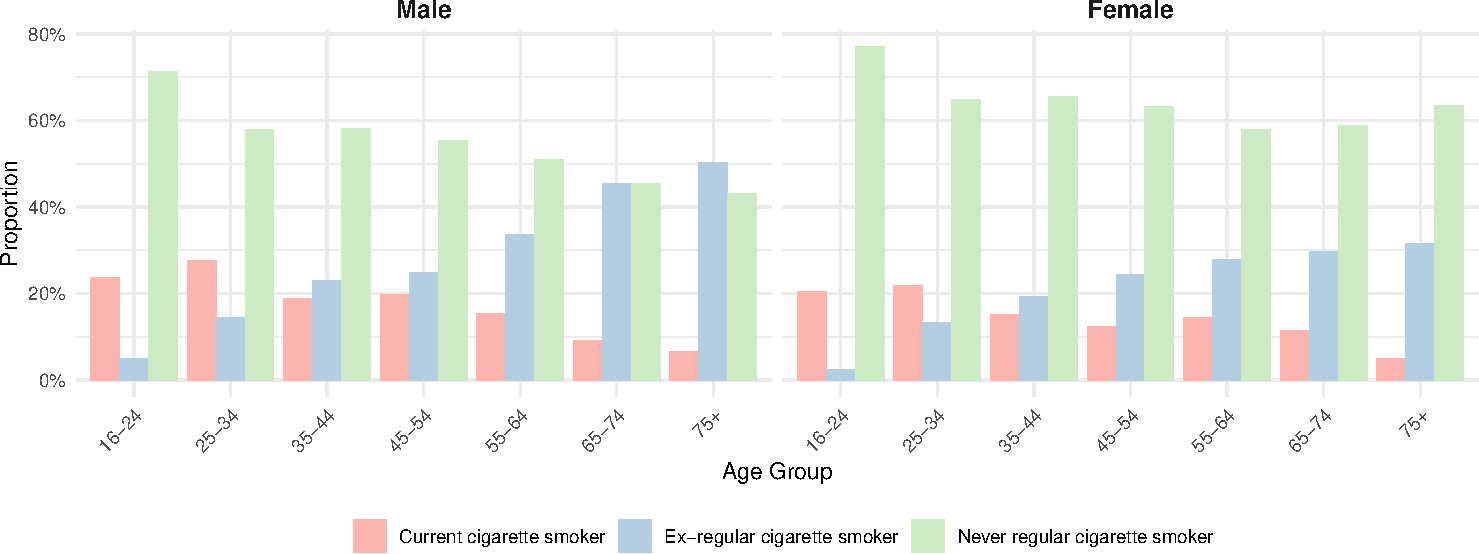
\includegraphics{Coursework_files/figure-latex/output smoking by age plot-1.pdf}
\caption{Smoking status proportions by age group and gender}
\end{figure}

\begin{figure}
\centering
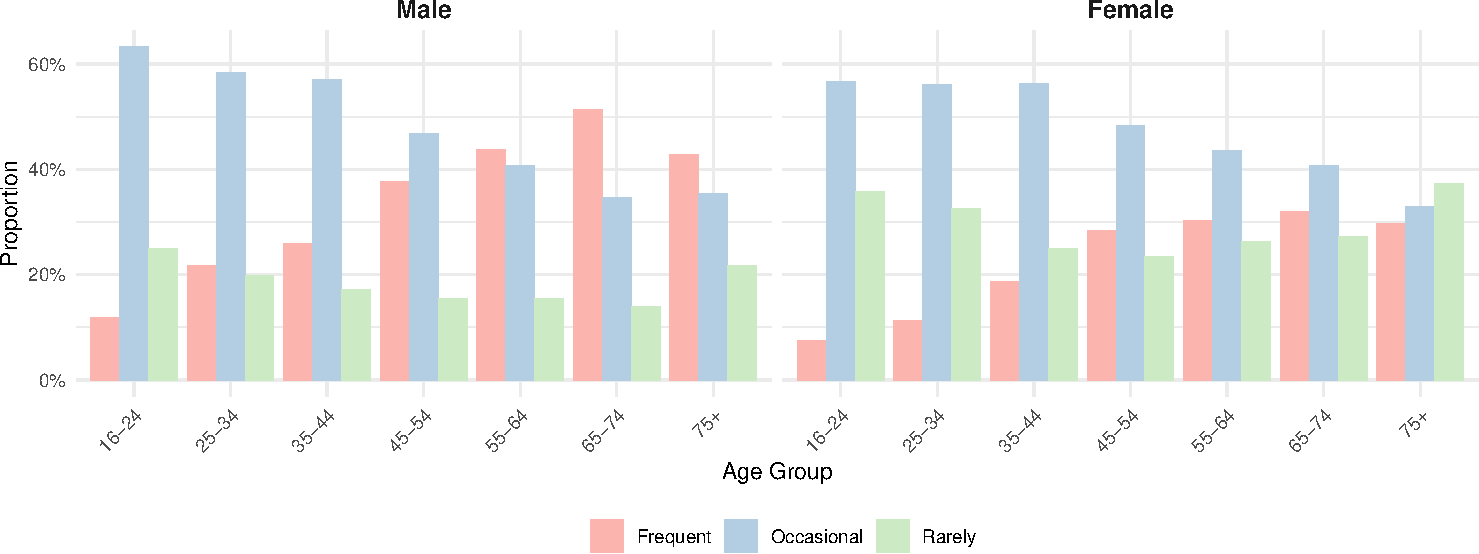
\includegraphics{Coursework_files/figure-latex/output drinking by age plot-1.pdf}
\caption{Drinking Status Proportions by age group and gender}
\end{figure}

\begin{figure}
\centering
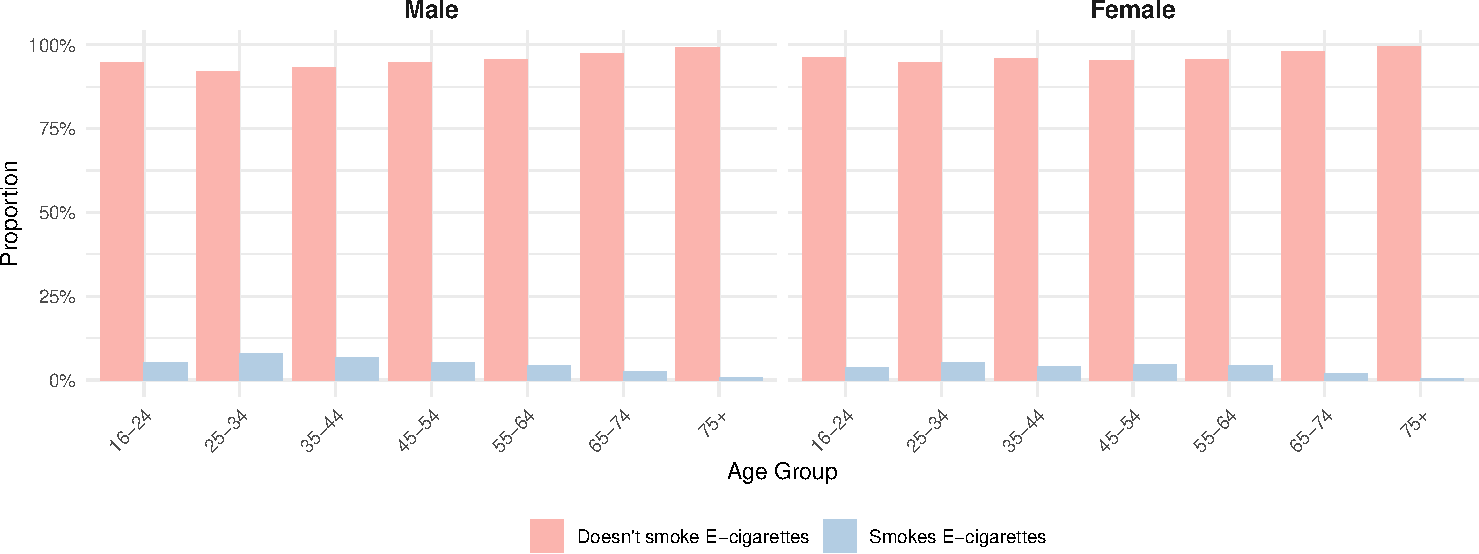
\includegraphics{Coursework_files/figure-latex/output e-cigs by age plot-1.pdf}
\caption{E-cigarette Usage Status Proportions by age group and gender}
\end{figure}

\begin{figure}
\centering
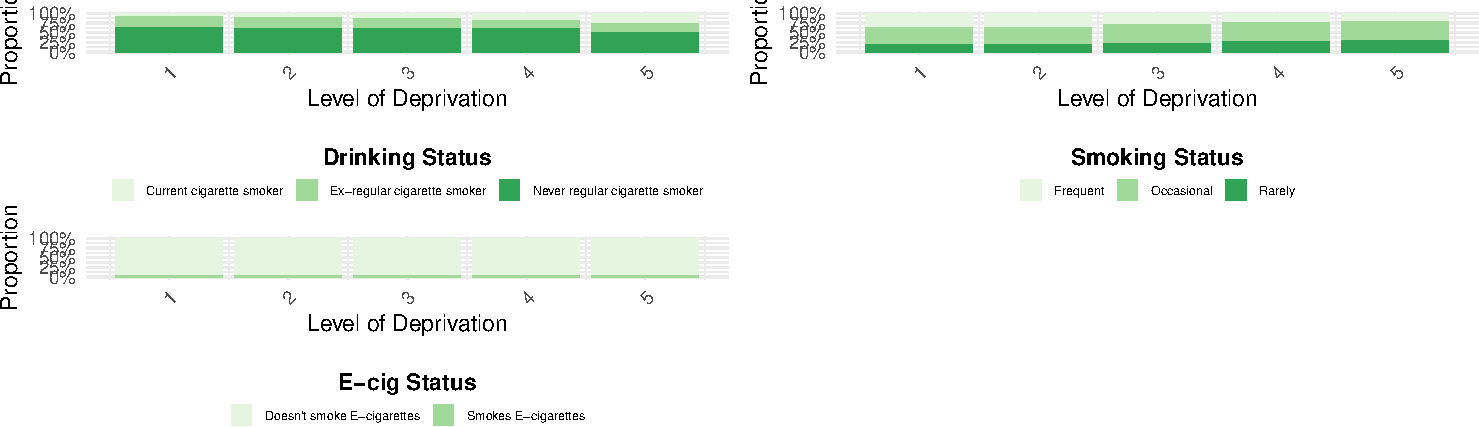
\includegraphics{Coursework_files/figure-latex/output deprivation plot-1.pdf}
\caption{Drinking Status Proportions by Level of Deprivation}
\end{figure}

Assuming a binomial\ldots{}

\begin{longtable}[]{@{}lll@{}}
\caption{Estimates and 95\% Confidence Intervals for \% of
Population}\tabularnewline
\toprule\noalign{}
Category & Estimate & C.I. \\
\midrule\noalign{}
\endfirsthead
\toprule\noalign{}
Category & Estimate & C.I. \\
\midrule\noalign{}
\endhead
\bottomrule\noalign{}
\endlastfoot
Drinking & 80.3\% & (79.5\%, 81.2\%) \\
Smoking & 16.5\% & (15.7\%, 17.3\%) \\
Smoking E-cigarettes & 4.28\% & (3.84\%, 4.72\%) \\
\end{longtable}

\begin{figure}
\centering
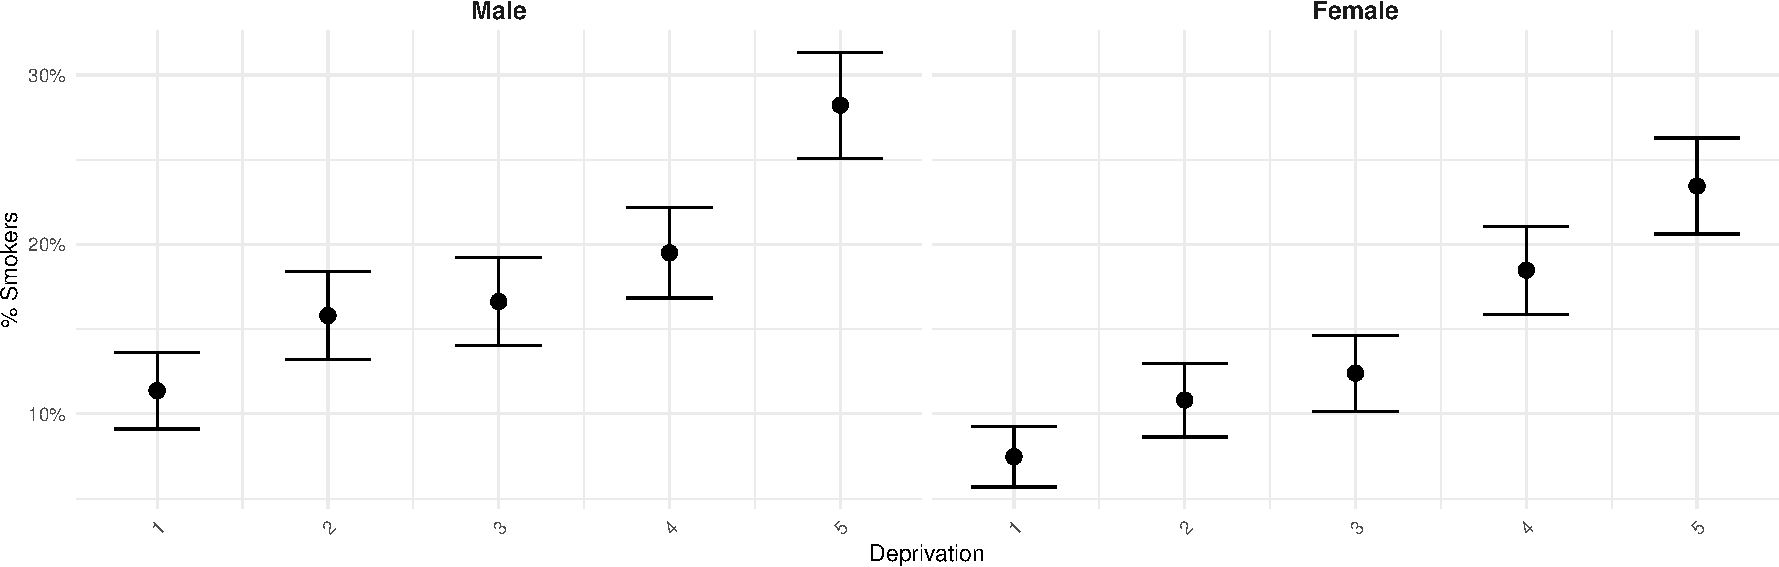
\includegraphics{Coursework_files/figure-latex/output prevelance plot-1.pdf}
\caption{Estimation of the prevelance of drinkers by city type and age
group}
\end{figure}

\section{Question Two}\label{question-two}

Explanation of why we split into test/train dataset.

This leaves us with 6563 observations in our training dataset.

\begin{longtable}[]{@{}lrl@{}}
\caption{Missing values in the training dataset}\tabularnewline
\toprule\noalign{}
Variable & Missing Values & \% Missing \\
\midrule\noalign{}
\endfirsthead
\toprule\noalign{}
Variable & Missing Values & \% Missing \\
\midrule\noalign{}
\endhead
\bottomrule\noalign{}
\endlastfoot
omsysval & 3216 & 49\% \\
dnoft\_19 & 1220 & 18.6\% \\
BMIVal & 1207 & 18.4\% \\
cigdyal\_19 & 49 & 0.747\% \\
cigsta3\_19 & 47 & 0.716\% \\
NDPNow\_19 & 44 & 0.67\% \\
d7many3\_19 & 43 & 0.655\% \\
drinkYN\_19 & 42 & 0.64\% \\
topqual2 & 36 & 0.549\% \\
origin2 & 24 & 0.366\% \\
marstatD & 1 & 0.0152\% \\
\end{longtable}

\end{document}
